\documentclass[10pt,a4paper]{article}
\usepackage[margin=2.2cm]{geometry}
\usepackage{fontspec}
\usepackage{kotex}
\setmainfont{Apple SD Gothic Neo}
\setsansfont{Apple SD Gothic Neo}
\usepackage{amsmath,amssymb}
\usepackage{graphicx}
\usepackage{caption}
\usepackage[dvipsnames]{xcolor}
\usepackage[colorlinks=true,linkcolor=MidnightBlue,citecolor=MidnightBlue,
            urlcolor=MidnightBlue]{hyperref}
\usepackage{titlesec}
\titleformat{\section}{\large\bfseries}{\thesection}{0.6em}{}
\captionsetup{font=small,labelfont=bf}
\setlength{\parskip}{0.35em}
\setlength{\parindent}{0pt}
\usepackage{mdframed}
\newmdenv[linewidth=0.4pt,linecolor=gray!60,backgroundcolor=gray!5,
          innertopmargin=6pt,innerbottommargin=6pt,skipabove=8pt,skipbelow=8pt]{claimbox}
\newcommand{\claim}[2]{\begin{claimbox}\textbf{주장.} #1\par\smallskip
  \textcolor{gray!70}{\textbf{반증 조건.} #2}\end{claimbox}}

\title{\bfseries 해로운 이름은 하나뿐이다 --- `만화'\\[2pt]
\large 이름 격자($3$짝 $\times$ $13$정체)가 법칙을 기각하고 더 단순한 것을 남겼다}
\author{월드모델 실험실 · 노트 $854$}
\date{2026-08-09}
\begin{document}\maketitle

\section{한 줄}

$853$ 의 `틀린 이름' 법칙에는 완전 교락이 있었다(틀린 이름 $2$짝이 둘 다 만화
원핫 --- 티처 \#$19$). 판별 셀을 포함한 전체 격자($3$평가짝 $\times$
$13$정체 · rankdata 해시 저장)를 재니: \textbf{KR 행에 게임 · 도서 · 모바일 ·
아이돌 등 어떤 `틀린' 이름을 붙여도 무해하고($0.388{\sim}0.394$ · 다수 셀은
무정체와 예측 완전 동일), 오직 `만화'만 $0.2561$($-0.136$)이다.} CN 도
만화가 최저, 앱$\times$만화도 $-0.018$. 법칙은 기각되고 더 단순한 사실이
남았다: \textbf{판의 $12$개 원핫 중 `만화'(JP · 판 최대 도메인)만이 판 밖
만화류 행에 강하게 --- 그리고 해롭게 --- 작용한다. 나머지 $11$개는 사실상
불활성이다.}

\begin{figure}[t]\centering
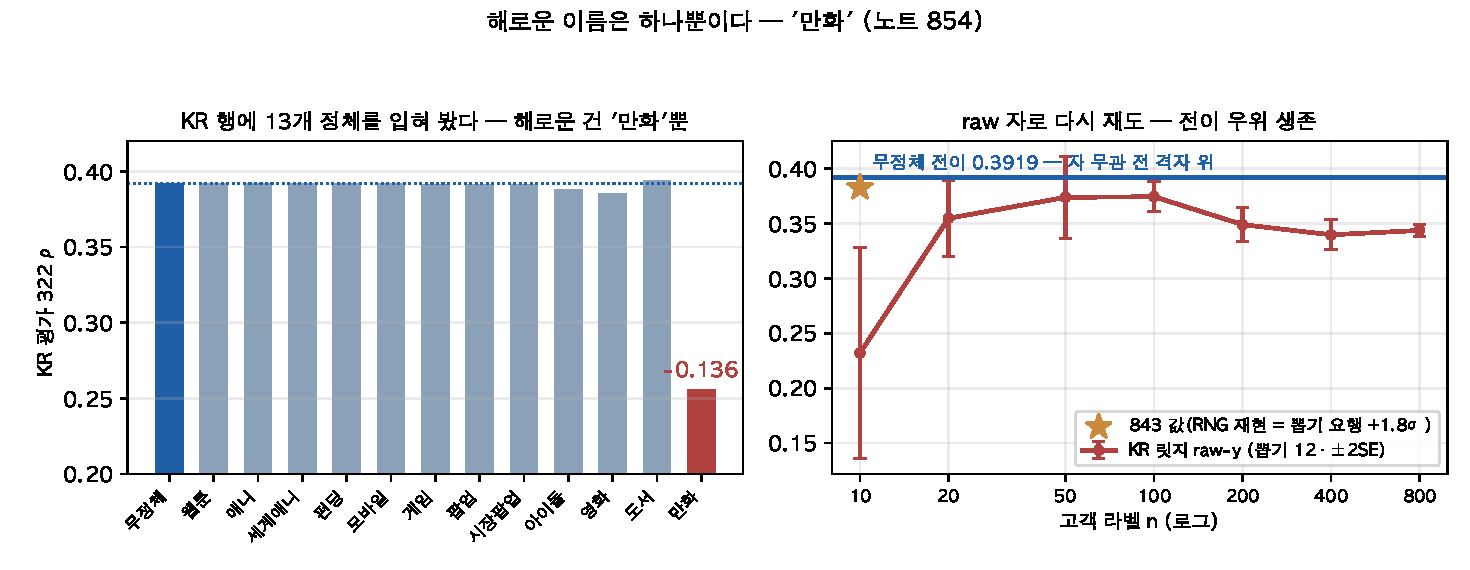
\includegraphics[width=0.97\textwidth]{figs/onename.pdf}
\caption{왼쪽: $13$개 정체 --- 해로운 건 `만화'뿐. 오른쪽: raw 자
재판정($12$뽑기)에도 전이 우위 생존.}
\end{figure}

\claim{\textbf{서빙 규칙이 최종 단순화됐다: 무정체 기본값 $+$ 판 밖 행에
`만화' 정체 부여 금지.} 그리고 릿지 대칭 재판정($12$뽑기 · raw/rank/raw-z ·
지문 y$+$pool)이 두 논쟁을 닫았다: ① $843$ 의 $0.3826$(KR $n{=}10$)은
\textbf{뽑기 요행($+1.8\sigma$)이 주범}이다 --- RNG 재현 팔이 $0.3826$ 을
정확히 재현했고(그 $4$뽑기는 실재하는 운 좋은 집합), $12$뽑기 raw 평균은
$0.232$, 목표 변환의 몫은 $+0.02$ 뿐. ② \textbf{KR 전이 우위는 자
무관}이다 --- raw 최강팔 최고점 $n{=}100$ 의 $0.3744{+}2$SE$=0.388 <
0.3919$(티처 \#$19$ 의 raw-미분리 우려가 $12$뽑기에서 해소). 앱은
$n^{\dagger}{=}50$ 확정($853$ 의 `$20{\sim}50$' 상단). 이득 지도 라우팅:
KR 는 라벨 $800$건까지 전이, 앱은 $50$건부터 로컬.}
{앱$\times$만화 해로움 $\ge 0.05$ 예측은 미스($-0.018$), KR raw$-$rank
$\ge 0.10$ 도 미스($+0.02$) --- $5/7$. 도서 원핫이 앱($+0.028$) · CN($+0.051$)
에서 무정체보다 낫다는 곁 관측은 다중비교 속 한 셀이라 해석하지 않는다.
왜 만화 원핫만 활성인지는 걸지 않는다(관측 후보만: 판 최대 도메인
$5{,}905$행이라 트리가 세게 학습).}

\section{정직}

$854$ 러너의 갈래 문구 `$843$ 재현 성공 $=$ 자 차 확정 · 요행 철회'는
오라벨이었다 --- 재현은 결정론의 확인일 뿐이고, 분해($12$뽑기 raw 대 rank)가
요행 주범을 확정했다. 이 정오를 본문으로 남긴다. CN 은 $19$행 참고
유지($853$ 의 갈래 결함 수정 이행). 봉인 $2$호 설계 동결(지문 · 타이브레이크
· 조용한 기본값 체크리스트). GitHub 흐름 $14$회째. 판 $\rho$ $0.4710$
그대로.

\end{document}
